\documentclass{ximera}  


\input{../preamble.tex}



 
\title{Electrostatic Potential} 
\author{Milica Markovic} 
\outcome{Electrostatic potential.}
\begin{document}  
\begin{abstract}  

\end{abstract}  
\maketitle    





\begin{dialogue}
\item[Petar] Potential? Another concept?
\item[Sasha] This one better be good.
\item[Petar] Look, it says here it is even simpler than Electric field because it is not a vector.
\item[Sasha] I'm all ears.
\end{dialogue}


\section{Electrostatic Potential Energy}


When charges are pushed around in electric field, the energy is not lost. Electrical forces are conservative. 


How much energy do we have to bring into system to bring two far-away positive charges at a distance r?

To answer that question, we can look at the Figure \ref{Potential1}. To bring the first charge to a certain position in space would require no work, since there are no other charged particles around, no electric field and therefore no force.  To bring the second charge at a distance r from the first charge, we need to overcome the repulsive force between the charges. How much work does this take? 
The work that we need to do to bring charges togehter is equal to the work that the first charge has to do to repel the second charge. The only difference is that we have to move the charges closer together, from infinity to some distance r, and the repulsive force does the work (pushes the charge $q_2$ away) from the distance r to infinity.



\begin{figure}[htbp]
\begin{center}
\includegraphics[scale=0.5]{../jpg/Two_Static_Charges_Potential.jpg}
\end{center}
\caption{Moving the charge $q_2$ with force $\vec{F}_{us}$ against the electrostatic force $\vec{F}_e$ due to charge $q_1$ to find the electrostatic potential energy} \label{Potential1}
\end{figure}


\begin{eqnarray}
W_{us}=W{e} \\
W_{us}= \int_{\infty}^{r} \vec{F}_{us} \cdot \vec{dr} \\
W_{e}=  \int_{r}^{\infty} \vec{F}_{e} \cdot \vec{dr} 
\end{eqnarray}

We know that the electric force $\vec{F}_e$, so we can calculate the total work necessary to bring the two charges at distance r.

\begin{eqnarray}
W_{us}= \int_{r}^{\infty} \vec{F}_{e} \cdot \vec{dr} \\
W_{us}= \int_{r}^{\infty} \frac{q_1 q_2}{4 \pi \epsilon_o r^2} \vec{r} \vec{dr}
\end{eqnarray}

Since the charge is moved in the  direction of the force, we can drop vectors, and calculate the work we have to do.

\begin{eqnarray}
W_{us}= \frac{q_1 q_2}{4 \pi \epsilon_o} \int_{r}^{\infty} \frac{dr}{r^2} \\
W_{us}=  \frac{q_1 q_2}{4 \pi \epsilon_o} (-\frac{1}{r}\Big|_{r}^{\infty})
W_{us}=  \frac{q_1 q_2}{4 \pi \epsilon_o r} \label{WorkPoinCharge}
\end{eqnarray}

This work is the same no matter what path we take to move charge $q_2$ from infinity to a distance r from charge $q_1$, see Figure \ref{PotentialWork}





\begin{figure}[htbp]
\begin{center}
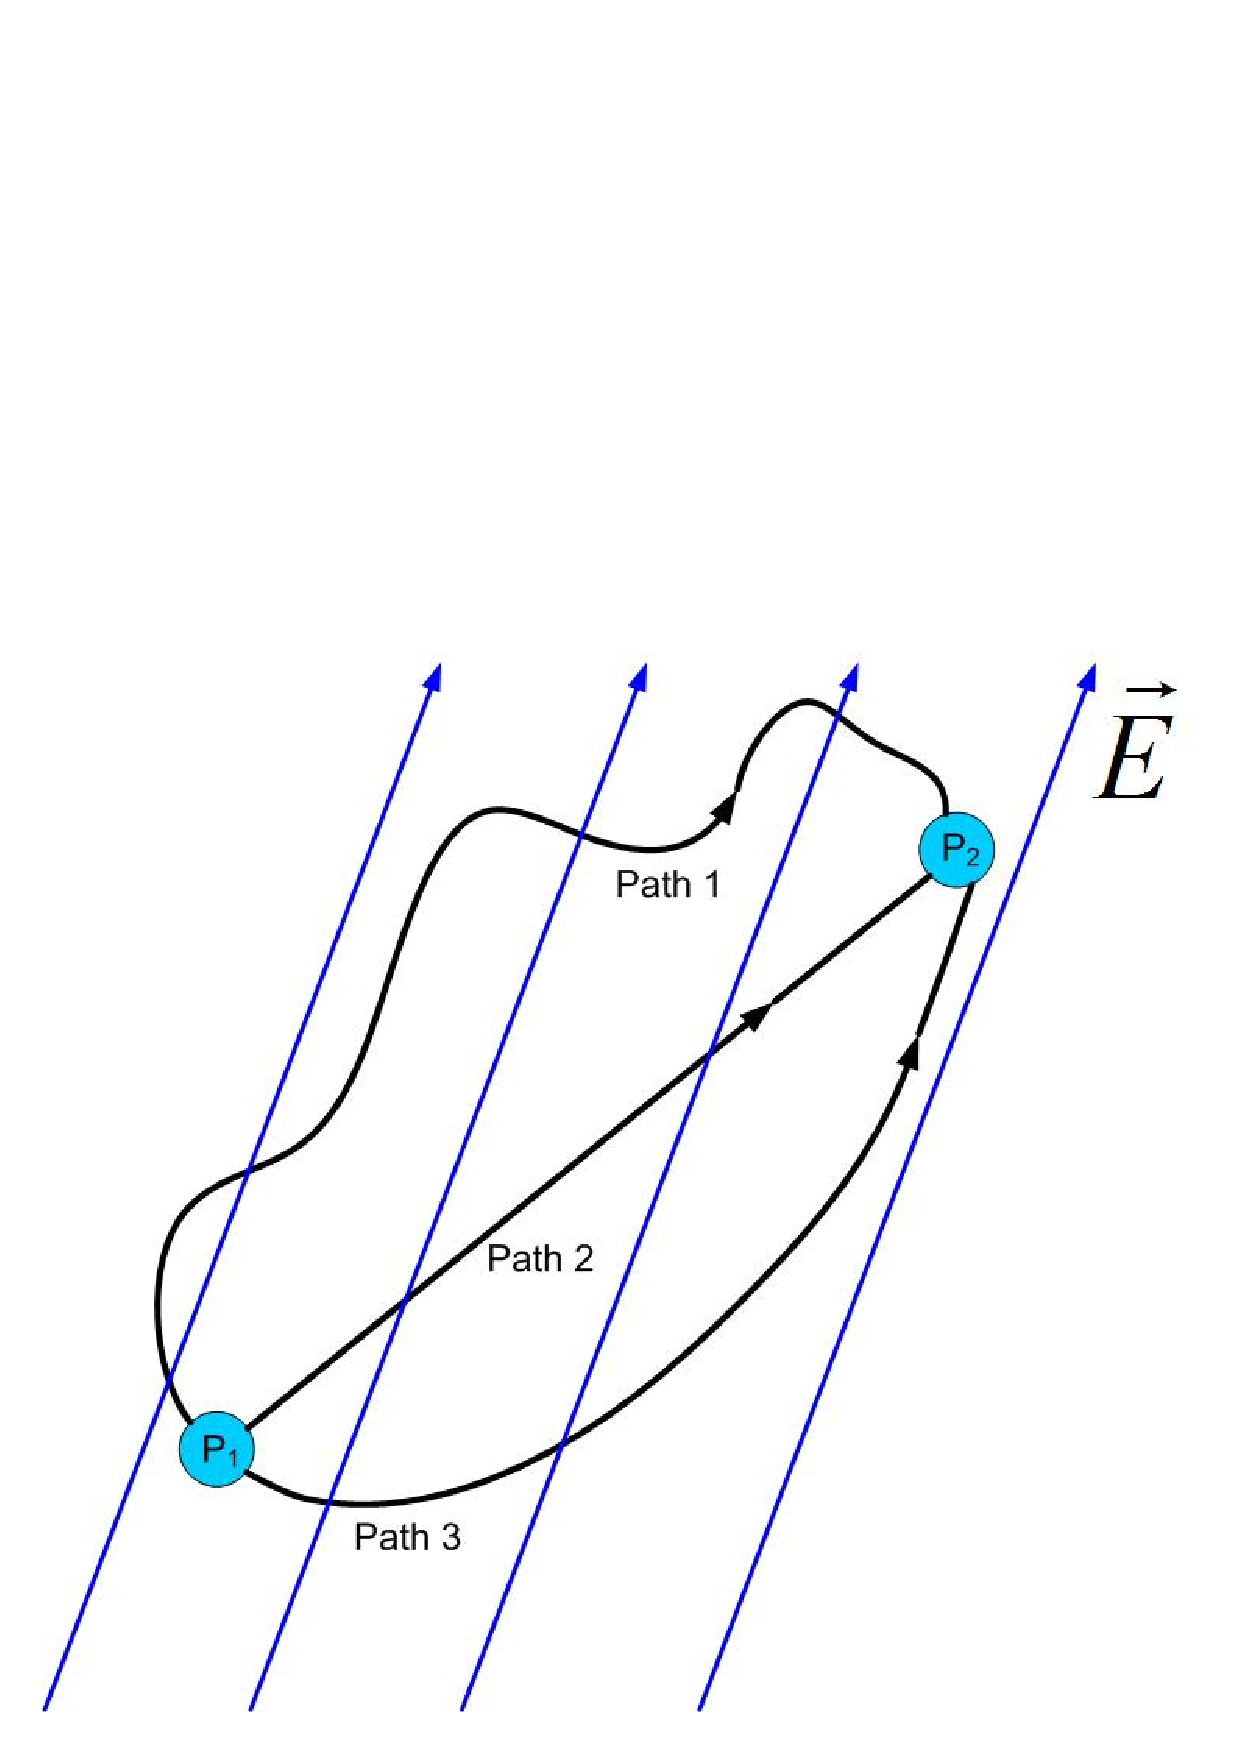
\includegraphics[scale=0.5]{../jpg/workindependentofpath.jpg}
\end{center} 
\caption{Potential is not dependent on the specific path.}\label{PotentialWork}
\end{figure}


\section{Definition of Potential and Voltage}


The work needed to move the two charges closer together depends on both charges $q_1$ and $q2$, just like the electrostatic force depends on both charges. It would be easier to define another variable that will separate the cause, charge $q_1$, and the effect, the work that we have to do to move charge $q_2$. This variable is Electric Potential. Electric potential is defined as the work we need to do to move the charge divided by the amount of charge $q_2$.

\begin{eqnarray}
V=\frac{W_{us}}{q_2} \\
V=\frac{q_1}{4 \pi \epsilon_o r} \label{Potential2}
\end{eqnarray}

Observe that in Equation \ref{Potential2} the potential is a function of the "source" charge $q_1$. We again separated the source and the effect, but this time of the potential energy. The source is a charge $q_1$ that produces potential V. If we now want to see what is the potential energy or work that we need to do to move another charge, we don't have to know which charge produced it, we only need to know the potential in an area, from which we can find the potential energy change of charge $q_2$. 

We can find a potential energy and potential of any number of charges using the above expression and the priciple of superposition. 













{\large EXAMPLE} Potential due to unit charge



\subsection{Electric Field inside Metals}





\begin{figure}[htbp]
\begin{center}
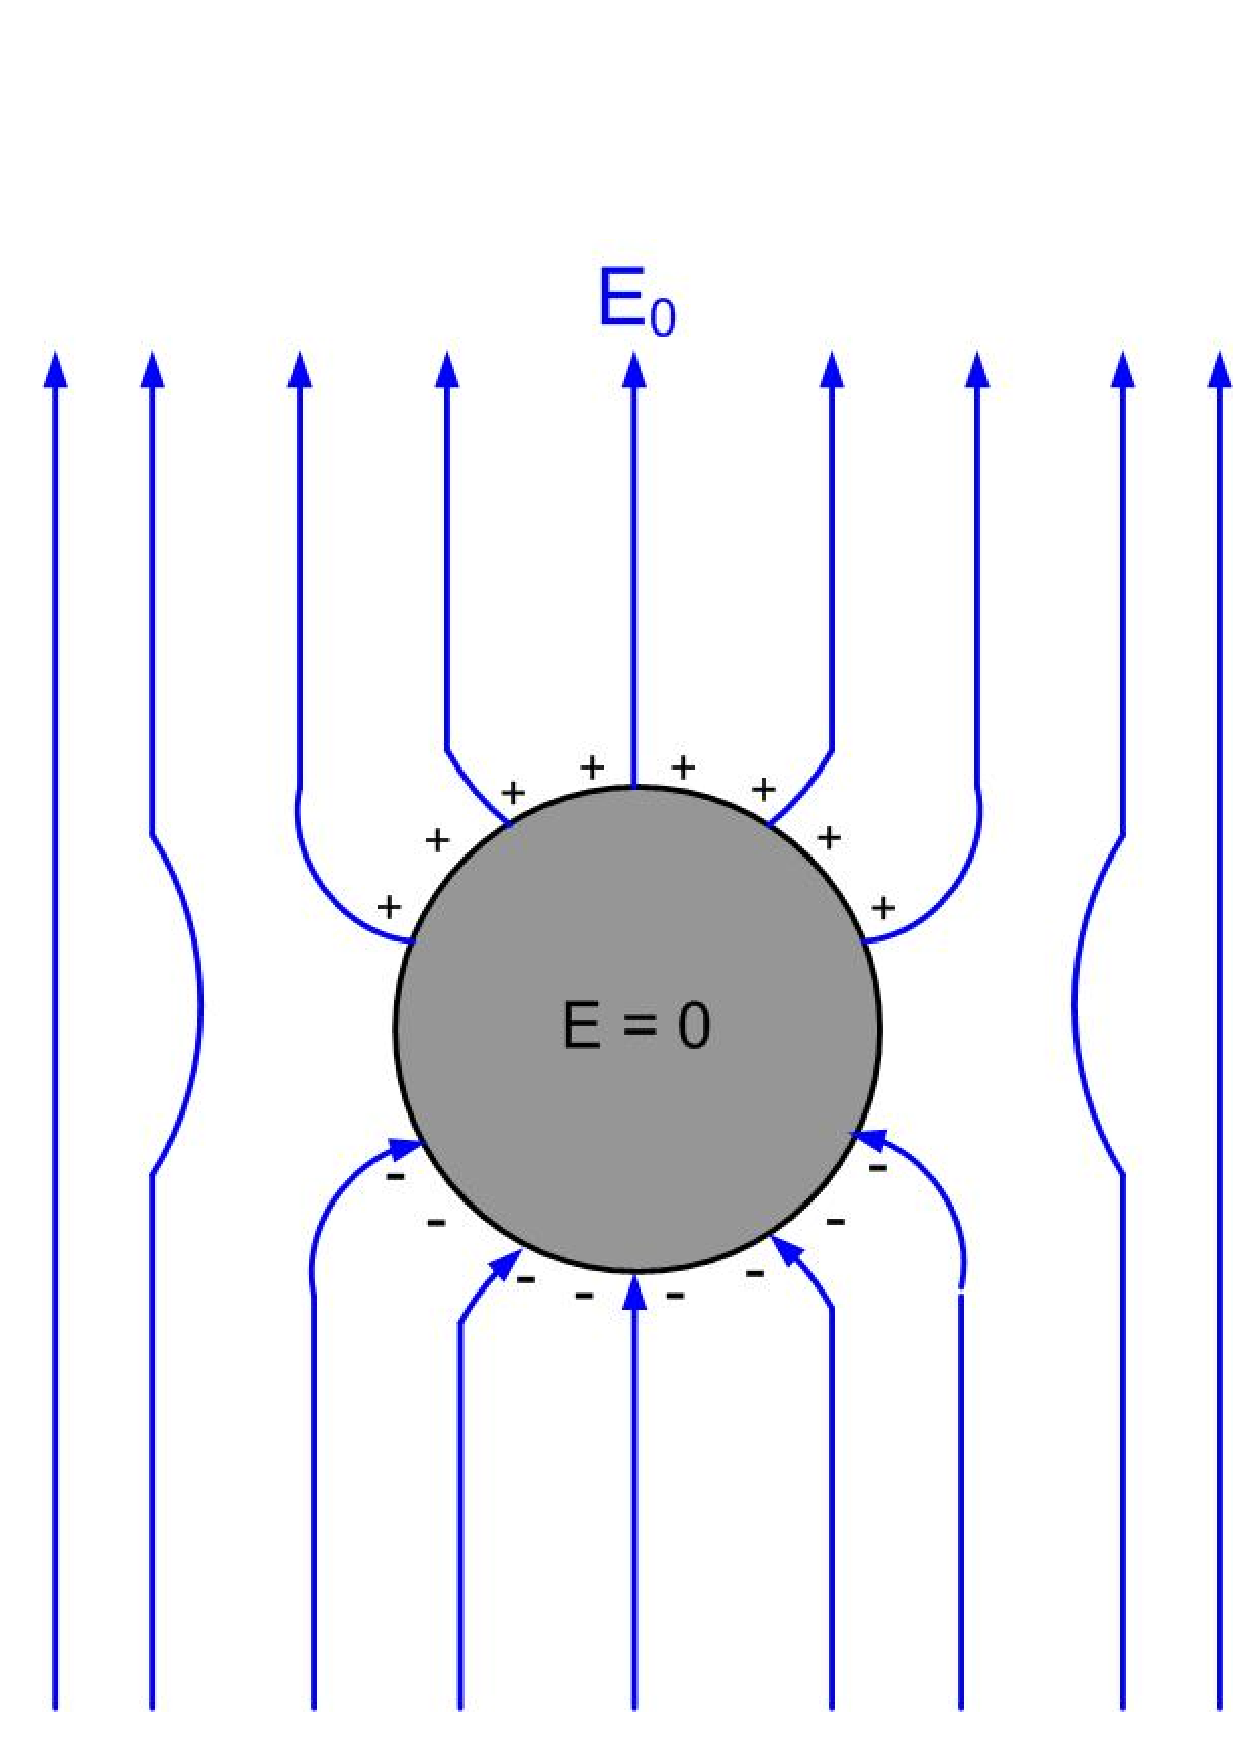
\includegraphics[scale=0.5]{../jpg/metalsphereinefield.jpg}
\end{center}
\caption{Metallic sphere in an external electric field.}
\label{BoundaryConditionMetal}
\end{figure}









\end{document} 
